% Klassifiziert den Dokumenten-Typ
% Doku: http://exp1.fkp.physik.tu-darmstadt.de/tuddesign/
% Farben: http://www.tu-darmstadt.de/media/medien_stabsstelle_km/services/medien_cd/das_bild_der_tu_darmstadt.pdf
%  bigchapter: Chapter haben doppelte Schriftgröße
%  linedtoc: Linien im Inhaltsverzeichnis wie bei Überschriften
%  colorbacktitle: Der Dokumenten-Titel wird mir der Accentfarbe hinterlegt
\documentclass[bigchapter,colorback,accentcolor=tud4b,linedtoc,11pt]{tudreport}

% Input Dokument hat das Encoding UTF-8
\usepackage[utf8]{inputenc}
% Wichtiges Paket für Links und verlinktes Inhaltsverzeichnis
\usepackage{hhline}
\usepackage[ngerman]{hyperref}
% Paket für Fußnoten
\usepackage[stable]{footmisc}
% Paket für amsmath (aligned mathe formeln)
\usepackage{amsmath}
% Paket für Bibliotheks-Verzeichnis, square: Verwende eckige statt runde klammern
% \usepackage[square]{natbib}
% Paket zum Plotten von Datensätzen
\usepackage{pgfplots}
\usepgfplotslibrary{patchplots}


\pgfkeys{%
  /pgfplots/default/.style={%
    /pgf/number format/use comma,
    legend pos=north west,
    width=0.9\linewidth,
    height=0.7\linewidth,
    scale only axis,
    xmin=0,
    ymin=0,
    grid=both,
    tick align=outside,
    tickpos=left,
    minor x tick num=3,
    minor y tick num=3,
    minor grid style={dotted,thin},
  }
}

% Anhänge für Original-Messdaten
\usepackage{fancyvrb}

% redefine \VerbatimInput
\RecustomVerbatimCommand{\VerbatimInput}{VerbatimInput}%
{fontsize=\footnotesize,
 %
 frame=lines,  % top and bottom rule only
 framesep=2em, % separation between frame and text
 fontsize=\scriptsize,
 %
 labelposition=topline,
 %
 commandchars=\|\(\), % escape character and argument delimiters for
                      % commands within the verbatim
 commentchar=*        % comment character
}

% Polar Plots
\usetikzlibrary{pgfplots.polar}
% Verwende deutsche Bezeichner für Inhaltsverzeichnis, ... (ngerman = New German: neue Rechtschreibung)
\usepackage{ngerman}
% Deutsche Zahlen (entfernt z.B. das Leerzeichen nach einem Dezimal-Komma)
\usepackage{ziffer} 

\usepackage[verbose]{placeins}

%wegen Grafikverschiebung hinzugefügt
\usepackage{float}

%\usepackage{graphicx}
%\usepackage{caption}
\usepackage{subcaption} %Für subfigures

% PDF-Optionen
\hypersetup{%
  pdftitle={TU Darmstadt \- Physikalisches Praktikum für Fortgeschrittene},
  pdfauthor={Esra Bauer und Sören Link},
  pdfsubject={Versuch 2.3},
  pdfview=FitH,
}
% Nummeriere formeln in Subsections einzeln
% Kleines makro zur assymetrischen Fehlerangabe

% Entspricht-Zeichen
\usepackage{scalerel}

\newcommand\equalhat{%
\let\savearraystretch\arraystretch
\renewcommand\arraystretch{0.3}
\begin{array}{c}
\stretchto{
    \scalerel*[\widthof{=}]{\wedge}
    {\rule{1ex}{3ex}}%
}{0.5ex}\\ 
=%
\end{array}
\let\arraystretch\savearraystretch
}
%BEGINN TITELSEITE

\title{$\alpha$-Spektroskopie mit einem Halbleiterzähler}

\subtitle{Esra Bauer \\Sören Link}

\subsubtitle{Betreuer: Simon Frydrych \hfill Versuchsdatum: 15. Juni 2015}

\author{Esra Bauer, Sören Link}

%\settitlepicture{img/title.jpg}

\institution{Physikalisches Praktikum \\für Fortgeschrittene \\Versuch 2.3}

\date{\today}


%ENDE TITELSEITE

\begin{document}
%ANFANG DOKUMENT

%Titelseite einfügen
\maketitle

%Inhaltsverzeichnis einfügen
\tableofcontents

%ANFANG INHALT

\chapter{Einleitung}

In diesem Versuch geht es um die $\alpha$-Spektroskopie mit einem Halbleiterzähler, wir nehmen also mittels eines Halbleiterdetektors das Spektrum eines $\alpha$-Strahler (in diesem Fall $^{241}Am$) auf und kalibrieren die digitalisierte Messung anschließend auf die Energie einer als bekannt vorausgesetzten Linie. Im Versuch soll das Messsystem Halbleiterzähler verstanden und angewendet werden, sowie später auf dieser Basis der Energieverlust geladener Teilchen in Materie bestimmt werden (hier: $\alpha$-Teilchen in Luft).

\chapter{Grundlagen}

\section{$\alpha$-Zerfall}

Alphazerfall ist eine Art des radioaktiven Zerfalls von Atomkernen. Der zerfallende Atomkern sendet einen Helium-4-Atomkern aus (Alphateilchen), wodurch die Massezahl des Mutterkerns um vier Einheiten un die Kernladungszahl um zwei Einheiten abnimmt. Beim Zerfall wird kinetische Energie frei, welche sich im umgekehrten Verhältnis der beiden Massen verteilt. Das Alphateilchen erfährt die attraktive starke Wechselwirkung, die eine kurze Reichweite besitzt, sowie Repulsion durch das Coulombpotential. Zusätzlich muss die Auswirkung des Kerndrehimpulses berücksichtigt werden. Durch den Zerfall wird die Energie des Teilchen in den quasigebundenen Bereich E > 0 angehoben, wodurch es mittels des quantenmechanischen Tunneleffektes das Coloumbpotential durchdringen kann. Mit Drehimpulskorrektur ergibt sich der folgende Hamiltonoperator: 
$$\hat{H} = \frac{-\hbar^2 \nabla^2}{2 m} – V_C(r) - \frac{l(l+1) \hbar^2}{2 m r^2},$$
wobei $V_C(r)$ das Coulombpotential ist und der letzte Term die Drehimpulskorrektur darstellt.
Der Transmissionskoeffizient ergibt sich als Quotient der transmittierten und der einlaufenden Betragsquadrate der Wellenfunktionen: $T = \frac{|\psi_t|^2}{|\psi_e|^2}$, was sich mit der Lösung der Schrödingergleichung schreiben lässt als $T \approx e^G$, wobei der sogenannte Gamow-Faktor G gegeben ist durch:
$$G = \frac{2 \sqrt{2 m}}{\hbar}\int_R^{R'} \sqrt{\frac{Z_1Z_2e^2}{r}-E} dr.$$

Alphastrahlung ist zur Spektroskopie insofern geeignet, als dass jedes Isotop Linien charakteristischer Energie und Intensität besitzt. Bei dem hier verwendeten Americium $^{241}Am$, welches ein reiner Alphastrahler ist, treten fünf verschiedene Linien auf, welche im Folgenden aufgelistet sind: 

\begin{center}
  \begin{tabular}{|p{5cm}|p{5cm}|}
    \hline
    E in keV & Intensität \\ \hline
    5388,23 & 0,016   \\ \hline
    5442,8 & 0,13   \\ \hline
    5485,56 & 0,845  \\ \hline
    5511,47 & 0,0022  \\ \hline
    5544,5 & 0,0034  \\ \hline
        \end{tabular}
\end{center}

Die mittlere Lebensdauer des Isotops beträgt 421,1 Jahre.

\section{Energieverlust geladener Teilchen in Materie}

Da Alphateilchen eine relativ große Masse und eine elektrische Ladung besitzen und eine viel höhere Ionisationsdichte als z.B. Beta- oder Gammastrahlung, ist ihre Eindringtiefe in Materie gering. Durch inelastische Stöße mit den Hüllenelektronen des Materials verlieren sie Energie. In Luft beträgt die Reichweite bei Normaldruck etwa 10 cm. Für den differentiellen Energieverlust schneller geladener Teilchen gilt die Bethe-Bloch-Gleichung, deren relativistische Form wie folgt lautet:
$$ - \frac{\mathrm{d}E}{\mathrm{d}x} = \frac{4 \pi nz^2}{m_{\rm e} c^2 \beta^2 } \cdot \left(\frac{e^2}{4\pi\varepsilon_0}\right)^2 \cdot \left[\ln \left(\frac{2m_{\rm e} c^2 \beta^2}{I \cdot (1-\beta^2)}\right) - \beta^2\right]$$
mit $\beta = \frac{v}{c}$, der mittleren Ionisationsenergie $I = kZ$ und der Elektronendichte $n = \frac{Z \rho}{A u}$, wobei Z und A Ordnungs- und Massezahl des Materials und $\rho$ dessen Dichte sind.
Für kleinere Geschwindigkeiten $v \ll c$ gilt folgende Näherung: 
$$- \frac{\mathrm{d}E}{\mathrm{d}x} = \frac{4 \pi nz^2}{m_e v^2}
\cdot \left(\frac{e^2}{4\pi\varepsilon_0}\right)^2
\cdot \ln \left(\frac{2m_e v^2 }{I}\right),$$
wobei diese jedoch nur gültig ist, wenn das Teilchen noch mindestens so schnell ist, dass es keine Hüllenelektronen mit sich führt.
Der Verlauf des Energieverlustes von Alphateilchen in Luft ist durch die Bragg-Kurve gegeben und zeigt gegen Ende, d.h. kurz vor Stillstand der Teilchen, einen deutlichen Peak.

\section{Halbleiterdetektor}

Um den Halbzeiterzähler zu erklären, ist es sinnvoll, sich einige grundlegende Eigenschaften von Halbleitern in Erinnerung zu rufen. Wir betrachten das Bändermodell, da durch Superposition der Atomorbitale die erlaubten Energieniveaus jeweils leicht nach oben und unten wandern und somit zu Energiebändern verschmieren bzw. die Lösung der Schrödingergleichung für ein einzelnes Elektron durch das Feld der Ionenrümpfe aufweicht. Bei Halbleitern sind Valenz- und Leitungsband durch eine schmale Bandlücke von einigen eV voneinander getrennt und dazwischen befindet sich die Fermi-Energie. Beispielsweise durch thermische Energiezufuhr oder Absorption eines Photons kann ein Elektron die Bandlücke überwinden und ins Leitungsband gelangen, was zu einem Defektelektron oder Loch im Valenzband führt. Sowohl Löcher als auch Elektronen sind bewegliche Ladungsträger und sind für die elektrische Leitfähigkeit  verantworlich. Die intrinsische Leitfähigkeit des Halbleiters ohne Dotierung wird als Eigenleitfähigkeit bezeichnet. Sie nimmt mit der Temperatur zu. Um die Fermi-Energie eines Halbleiters zu verschieben, bietet sich die Dotierung an. Dabei wird der Halbleiter gezielt mit Elementen aus der dritten oder fünften Hauptgruppe verunreinigt. Aus der dritten Hauptgruppe entstammen Elektronenakzeptoren, d.h. obrhalb des Valenzbandes wird ein zusätzliches Energieband hinzugefügt, welches Elektronen aufnimmt. Das resultiert in positiver oder p-Dotierung, d.h. es überwiegt die Löcherleitung. Elemente aus der fünften Hauptgruppe dienen als Donatoren, d.h. knapp unterhalb des Leitungsbandes wird ein Elektronenspender hinzufügt und es überwiegt die Elektronenleitung (negative oder n-Dotierung). Bei beiden Dotierungsarten bleibt der Halbleiter allerdings nach außen elektrisch neutral.

Wenn nun ein p- und ein n-dotierter Halbleiter in Kontakt gebracht werden, bildet sich eine sogenannte Raumladungs- oder Verarmungszone aus. Zunächst diffundieren die freien Ladungsträger in das jeweils andere Halbleitermaterial und rekombinieren an der Grenzschicht. Dadurch bleiben Ionenrümpfe zurück, die im p-dotierten Halbleiter negativ geladen sind und positiv im n-dotierten. D.h. hierbei entsteht ein elektrisches Feld, welches der Diffusion entgegenwirkt und schließlich zum Gleichgewicht führt, wobei sich die Fermi-Energien der beiden Halbleiter angeglichen haben. Dies wird als Raumladungszone bezeichnet. Wird nun eine Spannung derart angelegt, dass der Minuspol am p-dotierten Halbleiter und der Pluspol am n-dotierten Halbleiter anliegen, vergrößert sich dieses elektrische Feld bzw. die Raumladungszone noch und es fließt nahezu kein Strom. In Durchlassrichtung (d.h. Minuspol an n-dotiertem und Pluspol an p-dotiertem Halbleiter) verkleinert sich die Raumladungszone und es fließt ein wesentlich größerer Strom.

Wir verwenden einen Oberflächensperrschichtdetektor, genauer einen p-n-Zähler mit Oberflächensperrschicht, d.h. einen p-dotierten Halbleiter, auf den eine n-dotierte Schicht aufgedampft ist, bei dem die positiv geladenen Alphateilchen auf die sich an der Oberfläche befindlichen Raumladungszone treffen und Elektron-Loch-Paare bilden, deren Anzahl der Energie der Teilchen proportional ist. Zunächst betrachten wir Oberflächenzustände. Wir können die Oberfläche eines Halbleiters definieren als diejenige Schicht, die andere Bindungsverhältnisse und -symmetrien besitzt als das Innere des Halbleiters. Es handelt sich um eine Schicht der Dicke nur weniger Atomlagen, in der weitere Energieniveaus im Bereich der Bandlücke auftreten. Falls genug solcher Zustände vorhanden sind, liegt die Fermi-Energie in diesem Bereich und es existieren folglich weitere Niveaus dicht über der Fermi-Energie, die die freien Ladungsträger des Halbleitervolumens aufzufüllen versuchen. 

In unserm Fall besteht der Halbleiterzähler aus Silizium, d.h. der Energieaufwand w zur Bildung eines Elektron-Loch-Paares beträgt 3,6 eV und ist somit deutlich höher als die Bandlücke (etwa 1 eV). Die Anzahl der gebildeten Paare ist dann gegeben durch $N = \frac{E}{w}$, die Schwankung beträgt $\Delta N = \sqrt{N F}$ mit dem sogenannten Fano-Faktor F, der das Verhältnis der realen Varianz mit der Varianz der Poisson-Verteilung angibt. Für die Poisson-Verteilung gilt, dass Erwartungswert und Varianz gleich sind. Für Silizium ist $F = 0,15$. Die Halbwertsbreite der Energie ist dann: $E_{FWHM} = 2,355 w \sqrt{N F} = 2,355 \sqrt{E w F}$.
Der Impulsanstieg ist eine Funktion, der von Energie, Richtung und Masse des einfallenden Teilchens sowie auch der Detektorbauart abhängt. Dies ist recht kompliziert, es lässt sich jedenfalls feststellen, dass die Impulsanstiegszeit für Oberflächensperrschichtdetektoren im Bereich von Nanosekunden liegt. Die Sammelzeit ist von den Ladungsträgerkonzentrationen im Halbleiter sowie von deren Beweglichkeit abhängig. Sie beträgt ebenfalls wenige Nanosekunden.

Da das Signal, welches der Detektor liefert, sehr schwach ist, muss es direkt hinter dem Detektor verstärkt werden, wofür wir einen Vorverstärker benutzen, der eine hohe Ladungssensitivität aufweist. Hierbei wird der Strom verstärkt und kann als Eingangssignal für den Spektroskopieverstärker genutzt werden, wo auch die Pulsformung erfolgt. Anschließend kann das Signal analog-digital konvertiert und auf dem Computer gespeichert werden. 

\chapter{Aufbau und Durchführung}

\section{Versuchsaufbau}
\begin{figure}[h] 
  \centering
     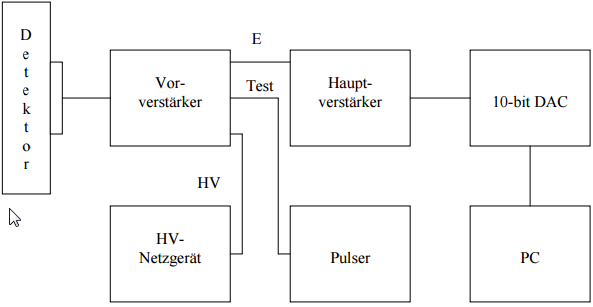
\includegraphics[width=0.8\textwidth]{img/Aufbau.png}
  \caption{Versuchsaufbau \cite{anleitung}}
  \label{fig:Bild1}
\end{figure}

\section{Durchfürhung}

\chapter{Auswertung}

\section{Kalibration der Energieskala}
\begin{figure}[h]
\begin{tikzpicture}
\begin{axis}[
    default,
    title={Kalibration des Halbleiterdetektors},
    xlabel=Kanal,
    ylabel=Counts,
    xmin=0,
    xmax=1024,
    ymode=log,
    ymin=1,
    ymax=100000,
    width=0.4\textwidth,
    height=0.4\textwidth
  ]
  \addplot[
  black, only marks, mark=+, mark size=2pt
  ] table[x expr=\coordindex+1, y index=0] {data/CALIBR.dat};
  \addlegendentry{Messpunkte}
  \addplot[red, mark=x, mark size=0pt, samples=100, domain=14:54] 
    {7011.605764712136/e^(0.29434965581444056*(-33.67872074878762 + x)^2)};
  \addplot[red, mark=x, mark size=0pt, samples=100, domain=118:158] 
    {7717.455825318301/e^(0.30789071693589276*(-138.25335222258695 + x)^2)};
  \addplot[red, mark=x, mark size=0pt, samples=100, domain=432:472] 
    {6904.329823546912/e^(0.31021660410784563*(-452.90210260199433 + x)^2)};
  \addplot[red, mark=x, mark size=0pt, samples=100, domain=948:988] 
    {13050.635733856781/e^(0.4405445287921415*(-968.7432082800937 + x)^2)};
  \addlegendentry{Peak-Fits}
\end{axis}
\end{tikzpicture}
%
\begin{tikzpicture}
\begin{axis}[
    default,
    title={Kalibration des Halbleiterdetektors},
    xlabel=Kanal,
    ylabel=Energie in $KeV$,
    xmin=0,
    xmax=1000,
    ymin=0,
    ymax=6000,
    width=0.4\textwidth,
    height=0.4\textwidth
  ]
  \addplot[black, only marks,mark=+, mark size=2pt, 
    error bars/.cd, y dir=both, y explicit
  ] table[x index=0, y index=1, y error index=2] {data/CALIBR-fitted.dat};
  \addlegendentry{Messpunkte}
  \addplot[red, mark=x, mark size=0pt, samples=100, domain=0:1000] 
    {357.4458819940879 + 5.294028183565216*x};
  \addlegendentry{Kalibrationsfit}
  \addplot[pink, mark=x, mark size=0pt, samples=100, domain=0:1000] 
    {357.4458819940879 + 5.294028183565216*x - 4.302652729749464* 
      (129.33390238062464 - 0.26700597705105833*x + 0.00013781903972842876*x^2)^0.5};
  \addplot[pink, mark=x, mark size=0pt, samples=100, domain=0:1000]
    {357.4458819940879 + 5.294028183565216*x + 4.302652729749464* 
      (129.33390238062464 - 0.26700597705105833*x + 0.00013781903972842876*x^2)^0.5};
  \addlegendentry{95\%-Fit}
\end{axis}
\end{tikzpicture}
\captionof{figure}{Kalibration}
\end{figure}

\section{Energie- und Intensitätsverteilung der $\alpha$-Linien}
\begin{figure}[h] 
  \centering
     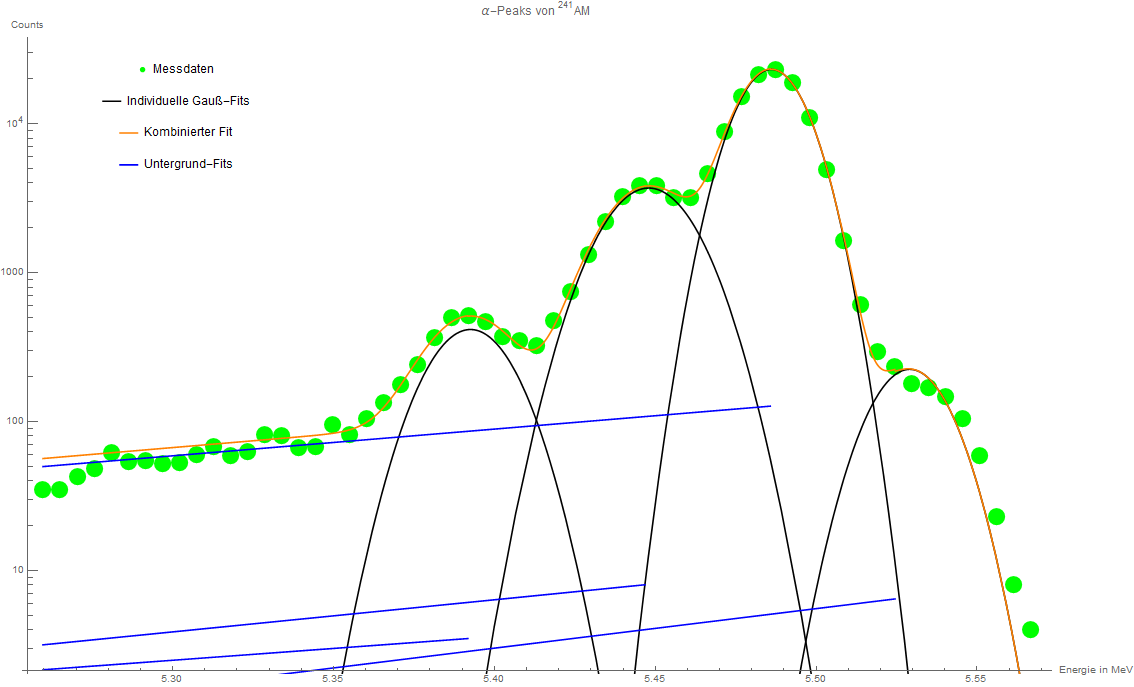
\includegraphics[width=1\textwidth]{img/alpha-spektrum.png}
  \caption{$\alpha$-Spektrum von $^{241}Am$ mit Untergrund, Gauß- und
    Summe aus allen Untergrund- und Gauß-Fits.}
  \label{fig:Bild1}
\end{figure}

\section{Energieverlust von $\alpha$-Strahlung in Luft}
\begin{figure}[H]
\begin{tikzpicture}
\begin{axis}[
  default,
  title={Kalibration des sekundären Thermometers},
  xlabel=Kanal,
  ylabel=Counts,
  xmin=0,
  xmax=850,
  ymin=0,
  ymax=550,
  height=0.5\linewidth
]
\addplot[
  red, only marks, mark=+, mark size=1pt
%, error bars/.cd, y dir=both, y explicit, x dir=both, x fixed relative=0.005
] table[x expr=\coordindex+1, y index=0] {data/AIR.DAT};
\addlegendentry{Messpunkte}
%\addplot[teal, mark=x, mark size=0pt, samples=40, domain=1.4:4.4] {-151.706+753.243/x};
%\addlegendentry{Curie-Fit}
%\addplot[orange, mark=x, mark size=0pt, samples=40, domain=1.4:4.4] {-155.706+769.835/(0.0247+x)};
%\addlegendentry{Curie-Weiss-Fit}
\end{axis}
\end{tikzpicture}
    \caption{}
\end{figure}

\chapter{Fazit}
%ENDE INHALT
\cleardoublepage{}
% Eintrag fürs Inhaltsverzeichnis
\newpage
\begin{thebibliography}{100}
  \bibitem{anleitung} Versuchsanleitung zum Versuch Alpha-Spektroskopie, heruntergeladen am 28.06.2015 von der Homepage der TU Darmstadt
  \bibitem{wiki} Grafik aus dem Artikel ---, der freien Enzyklopädie am 21.6.2015 \url{}
  
\end{thebibliography}
\end{document}

%%% Local Variables:
%%% mode: latex
%%% TeX-master: t
%%% End:
